
\chapter{背景分析}

银行是生活中不可缺少的一个媒介,银行的业务在于,一方面,它以吸收存款的方式,把社会上闲置的货币资金和小额货币节余集中起来,%
然后以贷款的形式借给需要补充货币的人去使用。另一方面,银行为商品生产者和商人办理货币的收付、结算等业务,它又充当支付中介。%
总之,银行在财政金融中作用。

项目主要模拟了银行中排队的情况:在一个银行中,可能有若干个窗口提供不同的业务,开始排队候,没个窗口处理业务的时间又不一样。%
现在简化这个问题的模型:假设一个银行中只有{\kaishu 两个}窗口:\textsl{A, B},\textsl{A} 窗口处理业务的速度是 \textsl{B}%
窗口的{\kaishu 两倍},假设所有顾客{\kaishu 同时}到达,输出处理完业务的顾客的先后序号。

项目还假设了每位顾客用一个编号表示,奇数号的顾客到 \textsl{A} 窗口办理业务,%
偶数号的顾客到 \textsl{B} 窗口办理业务。
测试以数字序列的方式输入,第一个数字$N$代表所有顾客的数量,后面跟着的 $N$ 个编号代表先后进入队伍的顾客。输出的时候需要将办理完%
业务的顾客依次输出,且 \textsl{A, B} 窗口同时办理完业务的情况下,\textsl{A} 窗口的顾客先输出。\vspace{0.7 cm}\\

{
    \begin{figure}[H]
        \centering
        \tikzstyle{recNode} = [rectangle, draw, fill=white]
        \tikzstyle{redCircle} = [circle, draw, fill=red, text = white, font={\bfseries}]
        \tikzstyle{blueCircle} = [circle, draw, fill=blue, text = white, font={\bfseries}]
        \tikzstyle{window} = [rectangle, fill=black, draw, font={\bfseries \Large}, text=white, rounded corners]
	    %定义语句块的颜色,形状和边
	    \tikzstyle{test}=[diamond,aspect=2,draw]  
	    %定义条件块的形状,颜色
        \tikzstyle{point}=[coordinate,on grid,] 
        \begin{tikzpicture}%[node distance=10mm,auto,>=latex',thin,start chain=going below,every join/.style={norm},] 
            \node[window] (AW) {A窗口};
            \node[redCircle, right of=AW, node distance=30mm] (01) {01};
            \node[redCircle, right of=01, node distance=15mm] (03) {03};
            \node[redCircle, right of=03, node distance=15mm] (05) {05};
            \node[redCircle, right of=05, node distance=15mm] (07) {07};
            \node[redCircle, right of=07, node distance=15mm] (09) {09};
            \node[redCircle, right of=09, node distance=15mm] (...) {...};
            \node[window, below of=AW, node distance=25mm] (BW) {B窗口};
            \node[blueCircle, right of=BW, node distance=30mm] (02) {02};
            \node[blueCircle, right of=02, node distance=15mm] (04) {04};
            \node[blueCircle, right of=04, node distance=15mm] (06) {06};
            \node[blueCircle, right of=06, node distance=15mm] (...) {...};
        \end{tikzpicture}
        \caption{银行业务处理示意图}
    \end{figure}
}

\chapter{功能设计}

\section{题意转化}
本题是典型的{\kaishu 排队}问题,排队的情况下,到达队伍与离开队伍顺序的关系满足{\kaishu 先进先出(First in First Out)}原则,%
排队问题可以通过数据结构\textbf{队列}解决:将排队的人{\kaishu 压入队尾(Enqueue)},然后{\kaishu 从队首取出(Dequeue)}当前排队的客户。如下图所示:

\begin{figure}[H]
    \centering
    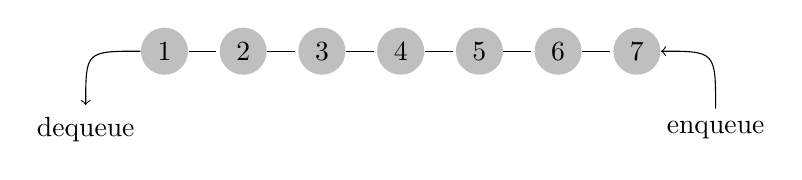
\begin{tikzpicture} [shorten >=1pt,
        vertex/.style={circle,fill=black!25,minimum size=17pt,inner sep=0pt}]
    \foreach \name/\x in {1/1, 2/2, 3/3, 4/4, 5/5, 6/6, 7/7}
        \node[vertex] (G-\name) at (\x,0) {$\name$};
    \foreach \from/\to in {1/2, 2/3, 3/4, 3/4, 4/5, 5/6, 6/7}
        \draw (G-\from) -- (G-\to);
    \node (de) at (0,-1) {dequeue};
    \node (en) at (8, -1) {enqueue};
    \draw [->] (G-1) .. controls (0,0) .. (de); 
    \draw [<-] (G-7) .. controls (8,0) .. (en);
    \end{tikzpicture}
    \caption{队列操作示意图}
\end{figure}

窗口 \textsl{A}、\textsl{B} 是两条不同的队列,因此题目中应该维护两个队列对象,由处理速度可知,当窗口 \textbf{A} 处理完%
两个业务后,窗口 \textsl{B} 才能处理完一个业务。

\vspace*{1cm}

\section{逻辑功能}
本题有两个窗口,所以在简单地将数据(客户)入队和出队的操作的基础上,还有两个重要的步骤:{\kaishu 判断窗口}和{\kaishu 决定出队顺序}。%

我们创建两个队列:\textbf{window A} 和 \textbf{window B}。在判断窗口的操作中,根据顾客编号值的奇偶性决定压入哪一个队列。%
在决定出队顺序时,以 \textbf{window A} 处理两个客户或者 \textbf{window B} 处理一个客户的时间为一个周期,%
每个周期开始时,先判断队伍是否有剩余客户,如果 \textbf{window A} 有客户则优先输出,%
\textbf{window A} 输出够两个或是为空之后再输出 \textbf{window B} 的一个客户。直到两个窗口均为空,处理结束。

\vspace*{2cm}

\section{流程图}

{
    \vspace*{2cm}
    \begin{figure}[H]
        \centering
        \tikzstyle{startstop} = [rectangle, rounded corners, minimum width = 2cm, 
                                 minimum height=1cm, text centered, draw = black, fill = red!40,
                                 font = {\bfseries}]
        \tikzstyle{io} = [trapezium, trapezium left angle=70, trapezium right angle=110, 
                          minimum width=2cm, minimum height=1cm, text centered, draw=black, fill = blue!40]
        \tikzstyle{process} = [rectangle, minimum width=3cm, minimum height=1cm, text centered, draw=black, fill = yellow!50]
        \tikzstyle{condition} = [diamond, aspect = 3, text centered, draw=black, fill = green!30]
        \tikzstyle{arr} = [->, >=stealth, thick]
        \begin{tikzpicture}
            \node (start) [startstop]  {开始};
            \node [io, below of = start, yshift = -1cm] (input) {输入};
            \node [process, below of = input, yshift = -1cm] (enqueue) {奇数入 \textbf{A},偶数入 \textbf{B}};
            \node [condition, below of = enqueue, yshift = -1cm] (condA) {\textbf{A} 为空?};
            \node [io, below of = condA, yshift = -1cm] (outA) {输出两个 \textbf{A} 中元素};
            \node [condition, below of = outA, yshift = -1cm] (condB) {\textbf{B} 为空?};
            \node [io, below of = condB, yshift = -1cm] (outB) {输出一个 \textbf{B} 中元素};
            \node [condition, below of = outB, yshift = -1.2cm] (condEnd) {\textbf{A}、\textbf{B} 均为空?};
            \node [startstop, below of = condEnd, yshift = -1.2cm] (end) {结束};

            \draw [arr] (start) -- (input);
            \draw [arr] (input) -- (enqueue);
            \draw [arr] (enqueue) -- (condA);
            \draw [arr] (condA) -- node[anchor=west] {是} (outA);
            \draw [arr] (outA) -- (condB);
            \draw [arr] (condB) -- node[anchor=west] {是} (outB);
            \draw [arr] (outB) -- (condEnd);
            \draw [arr] (condEnd) --  node[anchor=west] {是} (end);
            \draw [thick](condA) -- ($(condA.west) + (-2, 0)$) node (n) [anchor = east] {否} ;
            \draw [arr] (n.east) |- ($(condB.north) + (0, 0.5)$);
            \draw [arr] (condB) -- ($(condB.east) + (2, 0)$) node[anchor = west] {否} |- ($ (condEnd.north) + (0, 0.5) $);
            \draw [thick] (condEnd) -- ($(condEnd.west) + (-3, 0)$) node (n2) [anchor = east] {否};
            \draw [arr] (n2.east) |- ($(condA.north) + (0, 0.5)$);
        \end{tikzpicture}
        \caption{业务处理逻辑流程图}\label{yewu}
    \end{figure}
}
